%%This is a very basic article template.
%%There is just one section and two subsections.
\documentclass{scrartcl}
\usepackage[colorlinks, urlcolor=blue]{hyperref}
\usepackage{fullpage}
\usepackage{graphics}
\usepackage{graphicx}
\usepackage{verbatim}

\title{Ohmage Installation and Administration Manual for Ubuntu 12.04 (LTS)}
\subtitle{Version 2.14-0}


\begin{document}

\maketitle

\noindent Feedback, bugs, comments, suggestions, etc, about the Ubuntu
installation packages or this document are welcome and can go to
\href{mailto:jeroen.ooms@stat.ucla.edu}{jeroen.ooms@stat.ucla.edu}.
Communication about the Ohmage software itself is easiets through github:
\href{https://github.com/cens/ohmageServer}{https://github.com/cens/ohmageServer}.


\section*{About}

The following instructions will deploy a server with:

\begin{itemize}
  \item Ubuntu 12.04
  \item Ohmage 2.14
  \item OpenCPU 0.7 (optional)
\end{itemize}

\noindent The 12.04 version of Ubuntu ships with the following
software versions of third party Ohmage dependencies:

\begin{itemize}
  \item Linux kernel 3.2.0
  \item OpenJDK 6b24
  \item MySQL 5.5.22
  \item Apache 2.2.20 (includes \texttt{mod-proxy-ajp} and \texttt{mod-ssl})
  \item Tomcat 7.0.26
  \item Postfix 2.9.1 (used only by \texttt{ohmage-selfreg})
  \item R 2.15.2 (used only by \texttt{ohmage-viz})
\end{itemize}

\noindent Please note that at this point there are no official Ubuntu builds of
Ohmage. The Ohmage installation packages for Ubuntu are kindly provided by the
\texttt{OpenCPU} project.



\section{Installation}

This section will show how to install Ohmage on Ubuntu 12.04. The system
currently consists of 4 installation packages: \texttt{ohmage-server},
\texttt{ohmage-viz}, \texttt{ohmage-standalone} and \texttt{ohmage-selfreg}.
The \texttt{ohmage-server} package is the main package, which will install the
ohmage server and administration frontend. The \texttt{ohmage-viz} package
installs the optional vizualization server. In production settings, the
vizualization server should preferably run on a different server than
\texttt{ohmage-server}. However, to install both the Ohmage server and
vizualization server on one and the same machine, this is easiest done by
installing \texttt{ohmage-standalone}. The \texttt{ohmage-standalone} package
is a meta-package that will install both \texttt{ohmage-server} and
\texttt{ohmage-viz}, and automatically update the Ohmage server to use the
localhost vizualization server. \\

\noindent Finally installing the \texttt{ohmage-selfreg} package activates the
self-registration on the server. However, in order for self registration to
work properly, the server might need a valid domain name, and proper DNS
configuration. For more details, see section \ref{selfreg}.

\subsection{Installing Ubuntu 12.04}

\noindent The current build of Ohmage requires an Ubuntu 12.04 system. Any
version of Ubuntu will do, e.g. Ubuntu Desktop, Ubuntu Server, Kubuntu,
Edubuntu, etc. If you are already have an installed system, you can skip this
section. \\

\noindent The preferred way of running Ohmage is on a clean Ubuntu Server
edition. A copy of the Ubuntu Server installation disc ISO can be obtained from
the Ubuntu download page: \\

\url{http://www.ubuntu.com/download/server} \\

\noindent If you would like to run Ohmage on an Amazon EC2 server, the best way
is to use one of the official AMI's as provided by the ubuntu team: \\

\url{http://cloud-images.ubuntu.com/precise/current/} \\

\noindent Another possibility is to install a Ohmage on a virtual Ubuntu server
inside another OS. For example, the free VMware Player is available for Windows 
and Linux, and on OSX one can use parallels to run an Ubuntu server. This way
you can install Ubuntu and Ohmage safely on top of an existing system.

\subsection{Getting the system up-to-date}

\noindent Before begin installation of Ohmage, make sure you are running Ubuntu
12.04 (Precise) by entering:

\begin{verbatim}
    cat /etc/*release
\end{verbatim}
If it turns out the system is running an older version of Ubuntu, upgrade the OS
to 12.04 first. If the system is indeed 12.04, continue by updating the software
packages to the latest versions:

\begin{verbatim}
    sudo apt-get update
    sudo apt-get upgrade
\end{verbatim}
Once the system is up to date, you can begin installing Ohmage.

\subsection{Ohmage Installation}

Start by adding the \texttt{ohmage-2.14} package respository to our system:

\begin{verbatim}
    sudo apt-get install python-software-properties
    sudo add-apt-repository ppa:opencpu/ohmage-2.14
\end{verbatim}
The system will ask for confirmation on importing the public key. After the
repository has been added to the system, update the package list:

\begin{verbatim}
    sudo apt-get update
\end{verbatim}
Once this has succeeded ohmage can be installed. You have two options. To
install only the ohmage server and frontend, run:

\begin{verbatim}
    sudo apt-get install ohmage-server
\end{verbatim}
This will be sufficient to get started with Ohmage. If you want to install both
ohmage and the optional vizualization server you can install

\begin{verbatim}
    sudo apt-get install ohmage-standalone
\end{verbatim}
In the case you want to install \emph{only} the vizualization server, but not
Ohmage itself, run:
\begin{verbatim}
    sudo apt-get install ohmage-viz
\end{verbatim}
Note that all of these packages are compatible. For example, to upgrade from
\texttt{ohmage-server} to \texttt{ohmage-standalone} simply install the
latter and it will automatically make the appropriate changes. \\

\noindent Ohmage has many dependencies, and installation might take a while on
a vanilla server. During installation of \texttt{MySQL} (a dependency), the
system might ask for a password for the mysql root user. Make sure to enter a strong
password and write it down somewhere. You will not need it anymore during the
insallation though.\\

\noindent If the installation finished without any problems, it will display the
ip address of the host somewhere at the end of the output, which you can can
open in your browser and use to test the server. 

\subsection{Uninstall Ohmage}

If you want to remove Ohmage from a system, run:

\begin{verbatim}
    sudo apt-get purge ohmage-*
    sudo apt-get autoremove --purge
\end{verbatim}
Note that this will delete all data including the \texttt{ohmage} MySQL
database.

\section{Administration}

The \texttt{ohmage-server} packages installs 2 sites:

\begin{itemize}
  \item Ohmage Server: \url{http://example.com/app/config/read}
  \item Ohmage Front-end: \url{http://example.com/ohmage}
  \item OpenCPU: \url{http://example.com/R} (only available with
  \texttt{ohmage-viz})
\end{itemize}

If the \texttt{ohmage-viz} or \texttt{ohmage-standalone} package is installed,
the OpenCPU interface to \texttt{R} is also available:

\begin{itemize}
  \item OpenCPU: \url{http://example.com/R} 
\end{itemize}

After installation, visit the administration front-end to setup the
administrator account: \url{http://example.com/ohmage}. After a new
installation, one can authenticate using the default username and password
\texttt{ohmage.admin} with \texttt{ohmage.passwd}. At first login, you will
be prompted to change this password. By default, both http and https are
enabled. However, the https is served by a self-signed a.k.a. \emph{snakeoil}
SSL certificate, so the browser will give a warning about insecure encryption.
For more info see the section \ref{ssl} of this manual.

\subsection{Tomcat}

Ubuntu 12.04 ships with Tomat7. The Tomcat server only hosts the AJP1.3
prototcol on port 8009. Actual incoming HTTP and HTTPS are handled by Apache2
and proxied to Tomcat. To manage the Tomcat server do:

\begin{verbatim}
    sudo service tomcat7 {start | stop | restart}
\end{verbatim}
This command calls the \texttt{/etc/init.d/tomcat7} script which should usually
not be edited. Some global variables can be modified in
\texttt{/etc/default/tomcat7}. Tomcat configuration files, for example
\texttt{server.xml} are located at

\begin{verbatim}
    /etc/tomcat7/
\end{verbatim}
The tomcat7 log files \texttt{aw.log} and \texttt{catalina.out} are located
at

\begin{verbatim}
    /var/log/tomcat7/
\end{verbatim}
The \texttt{webapps} directory, hosting the \texttt{.war} files is located at

\begin{verbatim}
    /var/lib/tomcat7/webapps/
\end{verbatim}

\subsection{Apache2}

Incoming requests on port 80 (HTTP) and port 443 (HTTPS) are handled by the
Apache2 webserver. The \texttt{mod\textunderscore proxy\textunderscore ajp}
module is used to proxy requests to Tomcat server. To manage Apache2 use:

\begin{verbatim}
    sudo service apache2 {start | stop | restart}
\end{verbatim}
This command calls the \texttt{/etc/init.d/apache2} script which should usually not be edited. The main configuration file for apache2 is located at

\begin{verbatim}
    /etc/apache2/httpd.conf
\end{verbatim}
However by convention this file should rarely be edited. Custom configurations
are located at:

\begin{verbatim}
    /etc/apache2/mods-available/
    /etc/apache2/sites-available/
\end{verbatim}
These custom configurations can be activated and de-activated as follows:

\begin{verbatim}
    sudo a2enmod proxy_ajp
    sudo a2dismod proxy_ajp
    sudo a2ensite ohmage
    sudo a2dissite ohmage
\end{verbatim}
These commands create or remove symoblic inside links to available configuration
files inside the following directories:

\begin{verbatim}
    /etc/apache2/mods-enabled/
    /etc/apache2/sites-enabled/
\end{verbatim}
All files in these directories are automatically included by the main
\texttt{httpd.conf} file. The \texttt{ohmage} and \texttt{OpenCPU} sites are
defined in the following files:

\begin{verbatim}
    /etc/apache2/sites-available/ohmage
    /etc/apache2/sites-available/opencpu
\end{verbatim}
The Apache2 log files \texttt{access.log} and \texttt{error.log} are located at

\begin{verbatim}
    /var/log/apache2/
\end{verbatim}

\subsection{MySQL}

The MySQL server can be managed through:

\begin{verbatim}
    sudo service mysql {start|stop|restart}
\end{verbatim}

\noindent This command calls the \texttt{/etc/init.d/mysql} script which should
usually not be edited. Some global settings can be modified in
\texttt{/etc/mysql/debian-start} and \texttt{/etc/mysql/my.cnf}. In general, it
should not be required to manually enter mysql for using Ohmage. But if for some
reason you want to, you can connect to the mysql server using:

\begin{verbatim}
    mysql -u ohmage -p
\end{verbatim}
The password is \texttt{\&!sickly} and all ohmage data is stored in database
\texttt{ohmage}.

\subsection{OpenCPU (part of ohmage-viz)}

OpenCPU is used by the Ohmage-frontend to offer visualizations for data
exploration. If you do not plan on using data vizualization, or use an
external vizualization server, opencpu can be disabled:

\begin{verbatim}
    sudo a2dissite opencpu
\end{verbatim}
To change the vizualization server used by Ohmage, connect to MySQL and issue
the following command:

\begin{verbatim}
    use ohmage;
    update preference set p_value = "http://viz.example.com/R/call/Mobilize/"
    where p_key = "visualization_server_address";
\end{verbatim}
Where the server url is replaced by the appropriate viz server. To
restore it to the default value, run:

\begin{verbatim}
    use ohmage;
    update preference set p_value = "http://127.0.0.1/R/call/Mobilize/" where
    p_key = "visualization_server_address";
\end{verbatim}

\subsection{SSL certificate}
\label{ssl}

By default, Apache2 uses self signed a.k.a. snakeoil certificates. This is
convenient for development servers, but in a production setting these
should be replaced by SSL certificates signed by an official Certificate Authority. \\

\noindent The https configurations and locations of the certificates are defined
in

\begin{verbatim}
    /etc/apache2/sites-available/default-ssl
\end{verbatim}
This file also contains detailed comments with configuration instructions.

\subsection{Self registration}
\label{selfreg}

Ohmage supports option self registration. This means that users can register an 
account for themselves without any help from an administrator. The self
registration module can be installed as follows:

\begin{verbatim}
    sudo apt-get install ohmage-selfreg
\end{verbatim}

\noindent As part of the self registration process, a user will receive an email
with a confirmation code, and a link back to the server. In order for this to
work properly, the server needs a valid hostname. The hostname of the server is
defined in this file:

\begin{verbatim}
    /etc/hostname
\end{verbatim}

\noindent The link that is included in the confirmation email that self
registered user receive, is determined by this file, so make sure it contains a
proper hostname, and not e.g. \texttt{localhost} or some internal name. \\

\noindent The self registration depends on a properly functioning
SMTP server on the system, either Postfix or Sendmail. These will automatically
be installed when installing \texttt{ohmage-selfreg}. During the installation of
Postfix you might be propted for the hostname of your server. Again, make sure
that you enter a valid hostname here that can be reached through the internet.

\subsubsection{Important: Reverse DNS and Spam Detection}

Because spam is a big problem these days, most email providers tend to flag
emails that have been send from anonymous SMTP servers as spam. As a result,
the self registration confirmation emails might end up in their spam-folder or
junkmail. In order to minimize the chance that emails from Ohmage end up in spam
filters, it is highly recommended to use a domain that you actually purchased,
and not just the hostname of the machine that your ISP/hosting partner provided.
Furthermore it is important that the \emph{\textbf{reverse DNS}} of the server
to points back to this same domain name. Setting the reverse DNS is a process
that only your hosting provider can do for you. Most providers require you to
request this manually, for example, on EC2 you have to fill out this form: \\

{\footnotesize\url{https://aws-portal.amazon.com/gp/aws/html-forms-controller/contactus/ec2-email-limit-rdns-request}}
\\



\noindent In order to test if the the DNS and Reverse DNS are working properly,
you can use a command like \texttt{nslookup} on Linux or \texttt{tracert} on
Windows. Alternatively you can use a free web tool to do the lookup for you,
for example \url{http://www.dnsgoodies.com/}.

 



\subsection{Other Ohmage files}

Photos, videos and documents uploaded by users are stored in

\begin{verbatim}
    /var/lib/ohmage/images/
    /var/lib/ohmage/documents/
    /var/lib/ohmage/videos/
\end{verbatim}
Log files for ohmage can be found in:

\begin{verbatim}
    /opt/ohmage/logs
\end{verbatim}

\noindent Note that these are only high level ohmage logs. If there are problems
with the web server or database itsefl, these might appear in the tomcat logs. 
Finally, some static files included in the installation packages (scripts,
war files) can be found at:

\begin{verbatim}
    /usr/lib/ohmage/
\end{verbatim}

\section{Clients}

Currently there are 3 clients for the Ohmage server system. These are:

\begin{itemize}
  \item The Ohmage Android App.
  \item The Ohmage FrontEnd.
  \item The Ohmage R package.
\end{itemize}
Below a brief description of these clients.

\subsection{The Ohmage Android App}

The Ohmage Android 'app' is the application on the mobile phone that can be used
to fill out surveys and upload survey-responses to the server. As it currently
stands, the server-url is hardcoded in the app and therefore the app has to be
built from source. Figure \ref{fig:phone} shows a screenshot of the phone app running on
an Android 2.2 device. \\

\begin{figure}[h!]
\begin{center}
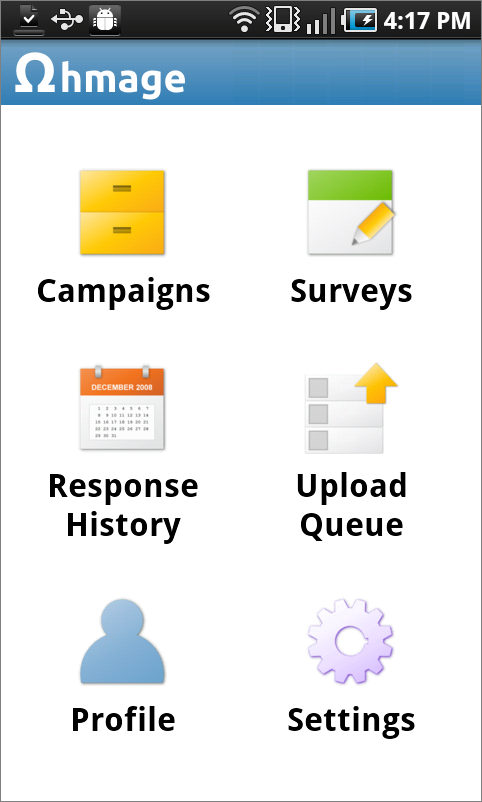
\includegraphics[width=4cm]{app.png}
\caption{A screenshot of the Android app.}
\label{fig:phone}
\end{center}
\end{figure}

\noindent The Android app can be downloaded from Google Play on any
Android phone by searching for \texttt{ohmage}. More information about the
app is available at: \\

\url{https://play.google.com/store/apps/details?id=org.ohmage} \\

When running the app for the first time after installing it from Google play, it
will prompt the user for the server address of the Ohmage server.
Alternatively, the app can be build from source. This way, the app can be
distributed with a hardcoded server address. The source code and instructions on
how to build the app are publicly available on: \\

\url{https://github.com/cens/ohmagePhone} \\

\subsection{The Ohmage FrontEnd}

The Ohmage FrontEnd is an administrative web application to be used on a regular
browser by both users and administrators of Ohmage. The application is
automatically installed when installing the server using instructions above and
available through: \url{http://example.com/ohmage}. Source code and
development of the FrontEnd is publicly available on github at
\url{https://github.com/cens/ohmageFrontEnd}. Figure \ref{fig:frontend} shows a
screenshot of the FrontEnd homepage after logging in. \\

\noindent The FrontEnd is a convenient client to review, share and explore data,
add/remove users, classes, campaigns, perform administrative tasks, etc. The
frontend can be build with some custom skinning options. The screenshot shows a build of
Ohmage with the default theme.

\begin{figure}[h!]
\begin{center}
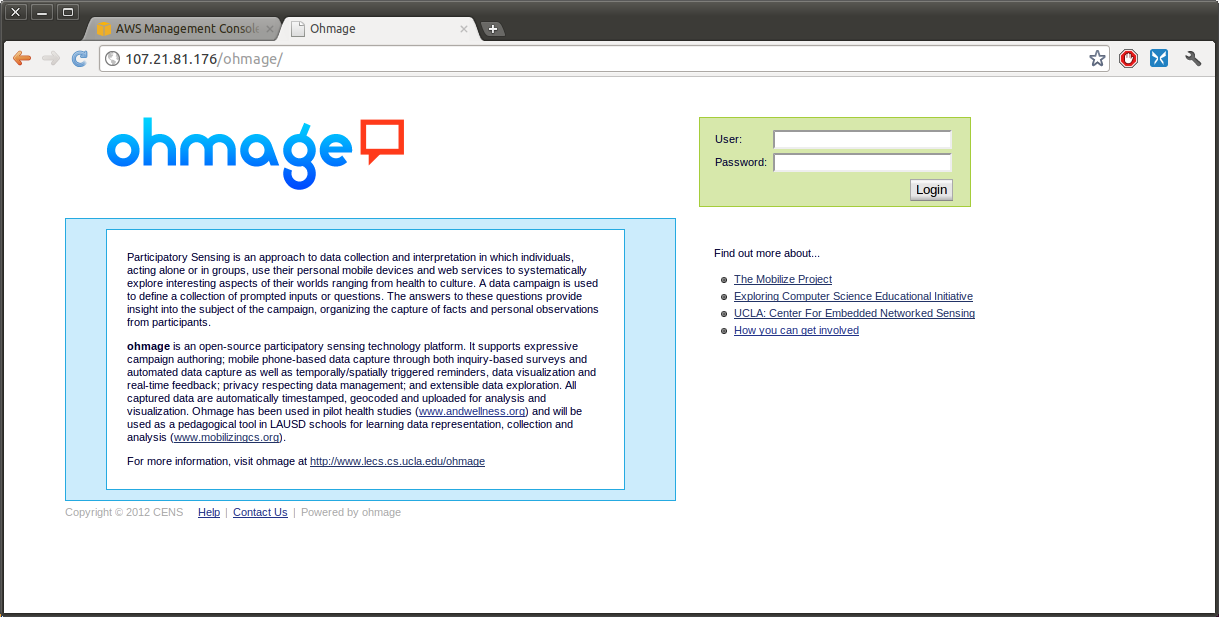
\includegraphics[width=15cm]{frontend.png}
\caption{A screenshot of the FrontEnd homepage.}
\label{fig:frontend}
\end{center}
\end{figure}

\subsection{The Ohmage \texttt{R} package}

The Ohmage R package is an Ohmage client for R. It depends on other R packages
like RCurl, XML and RJSONIO to do it's work. The package is mostly a convenient
way to grab data from Ohmage and turn it into a data frame in R. Package and
documentation are available from CRAN:
\url{http://cran.r-project.org/web/packages/Ohmage}. Below a code snippet to
illustrate the functionality of the package.

\begin{verbatim}
  library(Ohmage);
  oh.login("ohmage.admin", "mypassword", "https://myserver.com/app");
  campaigns <- oh.campaign.read();
  mydata <- oh.survey_response.read("urn:campaign:myschool:food");
\end{verbatim}

\section{Getting Started}

To understand how to use the Ohmage system, it is important to get familiar with
the basic concepts and terminology.  

\subsection{Survey terminology}

The Ohmage system is used for deploying surveys on mobile phones. These surveys
are defined in \emph{campaigns} using \texttt{XML} files. A user with
appropriate privileges can then upload such an XML file to the Ohmage server in
order to deploy the survey. Some essential concepts:

\begin{itemize}
  \item A \texttt{campaign} is an \texttt{XML} file which describes one or more
  \texttt{surveys}. 
  \item A \texttt{survey} is a set of survey questions called \texttt{prompts}.
  \item A \texttt{prompt} is a single question inside a survey. There are
  several \texttt{prompt types}. The prompt type specifies how the question is
  displayed in the phone, and how it is stored on the server.
\end{itemize}

\noindent A basic outline of the XML structure of a campaign is outlined below.

\begin{verbatim}
    <campaign>
      ... 
      <surveys>
        <survey>
          <id>snack</id>
          <title>snack survey</title>
          ...
          <prompt> ... </prompt>
          <prompt> ... </prompt>
          <prompt> ... </prompt>
        </survey>
        <survey>
          ...
        </survey>
      </surveys>
    </campaign>
\end{verbatim}

\noindent More details and examples on how to write a campaign can be found on
the wiki page:
\url{https://github.com/cens/ohmageServer/wiki/Campaign-Definition}.

\subsection{Users, Roles and Classes}
Users, roles and classes are the central concepts that control access to Ohmage.
A user is a person who can authenticate with the system and perform certain
actions. Users can either be created by an administrator, or self created,
when self registration is enabled on the server.\\

Users are organized in groups called \texttt{classes}. To give users access to a
campaign, the users has to be added to a class that is associated with this
campaign.\\

Permissions of users are defined using \texttt{roles}. There are two types of
roles: \texttt{class roles} and \texttt{campaign roles}. A user can have the
class role of \texttt{admin}, \texttt{privileged} or \texttt{restricted}. 
For each campaigns, the user can have any of the following roles:
\texttt{participant}, \texttt{analyst}, \texttt{author}, or \texttt{supervisor}.
For detailed descriptions on how classes and roles are used to manage user
access, consult this wiki page:\\

\url{https://github.com/cens/ohmageServer/wiki/About-Users,-Classes-and-Campaigns}



\subsection{Prompt types}

The prompt type is another central concept in the Ohmage system. Inside the XML
file, each survey lists one or more \texttt{prompts}. These prompts represent
survey questions. Each prompt has a \texttt{promptType} attribute, which defines
what kind of question this is. The promptType determines how the question is
displayed on the phone, how it is saved on the server, and what it looks like
when data is exported from the server. \\

Each prompt type has its own unique properties. These properties are used to
configure the question. The most important prompt types include:

\begin{itemize}
  \item \texttt{number} -- Displays a number field. Properties include
  \texttt{min} and \texttt{max}.
  \item \texttt{single\_choise} -- Displays a ``multiple choice'' radiobutton
  question with only one answer. Properties include a list of possible answers.
  \item \texttt{multi\_choice} -- Displays a ``multiple choice'' checkbox
  question where more than one answer can be checked. Properties include a list of
  possible ansers.
  \item \texttt{text} -- Displays a free text field.
  \item \texttt{photo} -- Allows the user to take a picture.
\end{itemize}

\noindent A more extensive list of different prompt types and their properties
is available here: \\

\url{https://github.com/cens/ohmageServer/wiki/Campaign-Definition#wiki-promptTypes}

\subsection{Work flow}

Below the steps that outline the work flow of using Ohmage. We assume the ohmage
server and front-end are installed using the \texttt{ohmage-server} package as
described in section 2.\\

\noindent The researcher first has to create a campaign and deploy it to the
users. These steps include:

\begin{enumerate}
  \item Write a campaign XML file that defines the survey questions.
  \item Deploy the XML on the server (using admin front-end)
  \item Create a class and associate it with the campaign (using admin
  front-end)
  \item Create ohmage user accounts for all participants and add them to
  the class.
  \item Notify your participants of the server address, and their
  username/password.
\end{enumerate}

\noindent Next, the participants can fill out the surveys

\begin{enumerate}
  \item Install the \texttt{ohmage} app on their phone.
  \item Login to the ohmage server with their username and password.
  \item Enroll in one of the campaigns they have access to.
  \item Fill out any survey as many times as desired.
\end{enumerate}

\noindent Finally, at any time the researcher can view and export responses from
the server. The administration front-end has some basic tools of exporting data
in e.g. CSV format.

\end{document}
